\documentclass[12pt, letterpaper] {article}

\parindent=5mm
\usepackage[spanish]{babel}

\usepackage{amssymb}
\usepackage{amsmath} 
\usepackage{amsfonts}

\usepackage[numbers,sort&compress]{natbib}
\usepackage{graphicx}

\usepackage{url}
\usepackage{hyperref}

\usepackage[top=25mm, bottom=20mm, left=1.5cm, right=1.5cm]{geometry}
\setlength{\parskip}{2mm}
\setlength{\parindent}{1pt}

\usepackage{listings}

\usepackage{float}

\usepackage[utf8]{inputenc}
\usepackage{graphicx} 
\usepackage{subfigure} 

\usepackage{color}
\usepackage{multirow}

\definecolor{dkgreen}{rgb}{0,0.6,0}
\definecolor{gray}{rgb}{0.5,0.5,0.5}
\definecolor{mauve}{rgb}{0.58,0,0.82}

\usepackage{color}
\usepackage{listings}
\lstset{ %
  language=R,                     % the language of the code
  basicstyle=\footnotesize,       % the size of the fonts that are used for the code
  numbers=left,                   % where to put the line-numbers
  numberstyle=\tiny\color{gray},  % the style that is used for the line-numbers
  stepnumber=1,                   % the step between two line-numbers. If it's 1, each line
                                  % will be numbered
  numbersep=5pt,                  % how far the line-numbers are from the code
  backgroundcolor=\color{white},  % choose the background color. You must add \usepackage{color}
  showspaces=false,               % show spaces adding particular underscores
  showstringspaces=false,         % underline spaces within strings
  showtabs=false,                 % show tabs within strings adding particular underscores
  frame=single,                   % adds a frame around the code
  rulecolor=\color{black},        % if not set, the frame-color may be changed on line-breaks within not-black text (e.g. commens (green here))
  tabsize=2,                      % sets default tabsize to 2 spaces
  captionpos=b,                   % sets the caption-position to bottom
  breaklines=true,                % sets automatic line breaking
  breakatwhitespace=false,        % sets if automatic breaks should only happen at whitespace
  title=\lstname,                 % show the filename of files included with \lstinputlisting;
                                  % also try caption instead of title
  keywordstyle=\color{blue},      % keyword style
  commentstyle=\color{dkgreen},   % comment style
  stringstyle=\color{mauve},      % string literal style
  escapeinside={\%*}{*)},         % if you want to add a comment within your code
  morekeywords={*,...}            % if you want to add more keywords to the set
} 

\usepackage{booktabs}
\usepackage[table,xcdraw]{xcolor}


\author{Ricardo Rosas Macías}

\title{Práctica 5: método Monte-Carlo}

\date{\today}

\begin{document}

\maketitle



\section{Introducción}

El método Monte Carlo es una herramienta matemática para calcular las probabilidades mediante una serie de números aleatorios, en virtud de ello nos permite identificar cuántos puntos se necesitan para estimar el valor de interés.

 \section{Objetivo}
En términos generales,  se realizó cambios en el código de modo que proporcionó el estimado en función de los decimales, para determinar el tamaño de muestra necesario para la aproximación del valor real.
 
 \subsection{Descripción}
 
Lo que se debe hacer es \cite{elisaweb}:
\begin{quotation}
 ``Determinar el tamaño de muestra requerido por cada lugar decimal de precisión del estimado obtenido para la integral, comparando con la calculadora virtual Wolfram Alpha \cite{Wol} de uno hasta siete decimales, asimismo representar el resultado como una sola gráfica.
 De igual manera para el primer reto, implementar la estimación del valor de $\pi$ de Kurt \cite{kurt} con paralelismo, determinar la relación matemática entre el número de muestras obtenidas y la precisión obtenida en términos de la cantidad de lugares decimales correctos''
\end{quotation}

\section{Resultados y conclusiones}

Para obtener los resultados se tomaron en base a la integral $\int _{ 3 }^{ 7 }{ f(x)dx }$ respecto a la función: $f\left(x \right)=\frac {1}{ \exp(x)\quad +\quad \exp(-x) }$.  Asimismo con los datos se realizó una normalización ($g(x)=2f(x)/\pi$) para obtener la distribución arbitraria, como se muestra en las siguientes líneas del código.\vspace{2mm}

\begin{lstlisting}[language=R]
desde <- 3
hasta <- 7
Pedazos <- 300
cuantos <- 100
muestra <- c(50, 100, 500, 1000, 5000, 10000)
wolfram<-0.048834 # Valor real
repeticiones <- 20
parte <- function() {
  val <- generador(pedazo)
  return(sum(val >= desde & val <= hasta))
}
Info <- data.frame()
for (pedazo in Pedazos) {
  for (cuantos in muestra){
    for (vez in 1:repeticiones){
      suppressMessages(library(doParallel))
      clust <- makeCluster(2)
      registerDoParallel(clust)
      montecarlo <- foreach(i = 1:cuantos, .combine=c) %dopar% parte()
      stopCluster(clust)
      integral <- sum(montecarlo) / (cuantos * pedazo)
      piInt <- (pi / 2) * integral
      pI <- c(piInt, cuantos, as.integer(pedazo))
      print(cuantos)
      Info <- rbind(Info, pI)
    }
  }
}
colnames(Info) <- c("val", "rep", "esp")
Info$esp <- as.integer(Info$esp)
Info$rep <- as.factor(Info$rep)
print(Info)

agregando <- function(Espacio){
  Espacio <- as.factor(Espacio)
  return(paste("n = ", Espacio, sep = ""))
}
valmin <- (wolfram-50)
\end{lstlisting}\vspace{-2mm}

El resultado final del código proporcionado muestra un valor aproximado que posteriormente se comparó con el valor real proporcionado de la calculadora Wolfram \cite{Wol}.
En la figura \ref{Apvreal} se observa la aproximación al valor real, en donde la secuencia de la muestra del experimento fue 300 realizando cambios en su tamaño; 50, 100, 500, 1000, 5000 y 10000, con 10 repeticiones para cada una. Esto nos permito conocer la aproximación  al valor real: 0.0488340. De manera que la gráfica nos muestra que al incrementar el tamaño de muestra la precisión incrementa en el resultado final, por lo tanto a 10000 la muestra tendrá mayor exactitud en los decimales del valor real, así como poca variación de los números aleatorios.

\begin{figure}[H]
\centering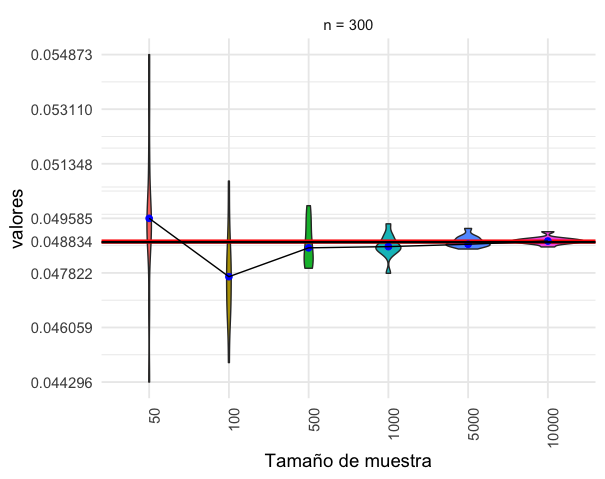
\includegraphics[width=120mm]{Aproxvalorreal.png}
\caption{Aproximación al valor real}
\label{Apvreal}
\end{figure}

\subsection{Reto 1}

De acuerdo a la ponderación anterior, para el primer reto se realizó el experimento a 10 repeticiones y con una secuencia de 300; en el cual las condiciones permitieron observar la aproximación de $\pi$ (3.14159265359), como se muestra en las siguientes líneas de código.

\begin{lstlisting}[language=R]
inicio <- -0.1
final <- -inicio
pi <- 3.14159265359
muestra <- c(10,50,100,500,1000)
repeticiones <- 30

calcpi=function() {
  xs <- runif(replicas, min= inicio, max= final)
  ys <- runif(replicas, min= inicio, max= final)
  in.circle <- xs^2 + ys^2 <= inicio^2
  mc.pi <- (sum(in.circle)/replicas)*4
  return(mc.pi) 
}
suppressMessages(library(doParallel)) 
registerDoParallel(makeCluster(detectCores() - 1)) 

resultados=data.frame() 

for(replicas in muestra) { 
  for(i in 1:repeticiones) { 
    montecarlo <- foreach(i = 1:300, .combine=c) %dopar% calcpi() 
    mc.pi=sum(montecarlo)/300
    diferencia=(pi-mc.pi)/(pi*100) 
    pii <- pi
    resultados=rbind(resultados,c(replicas,i,pii,mc.pi,diferencia))
  }
}
names(resultados)=c("muestra","replicas","Valor de Pi","aprox.pi","error") 
\end{lstlisting}

De modo que en la gráfica a de la figura \ref{Ret1} podemos notar que en comparación a los resultados anteriores hay una diferencia al tener un tamaño de muestra menor, este presenta una mejor aproximación al valor, como es el caso de la muestra 500; la cual denota un ligero cambio porcentual obtenido, así como su tamaño de error es ligeramente desapercibido en contraposición de las demás muestras.

\begin{figure}[H]
\centering
\subfigure[Aproximación a $\pi$]{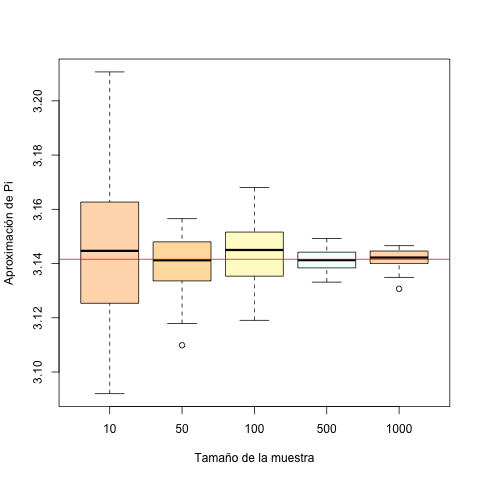
\includegraphics[width=88mm]{./Aproxr1}}\vspace{1mm}
\subfigure[Tamaño de error]{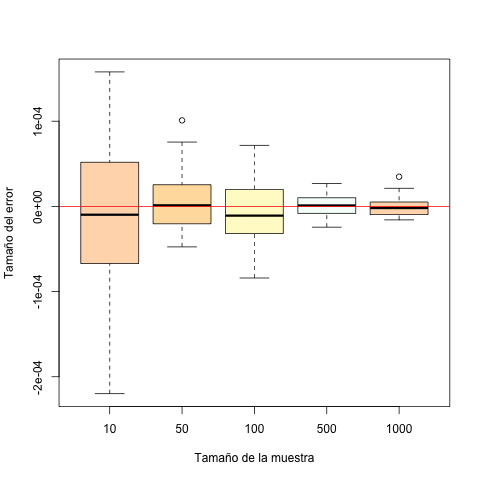
\includegraphics[width=88mm]{./Errorr1}}
\caption{Estimación al valor de $\pi$} \label{Ret1}
\end{figure}


\bibliographystyle{plainnat}

\bibliography{BHWP5}

\end{document} 